\subsection{\large{\textit{tI}8-YMn\textsubscript{2} (Direct)}}\vspace{-0.1in}
Manganese Yttrium


\begin{figure}[H]
\begin{minipage}{0.34\textwidth}\centering
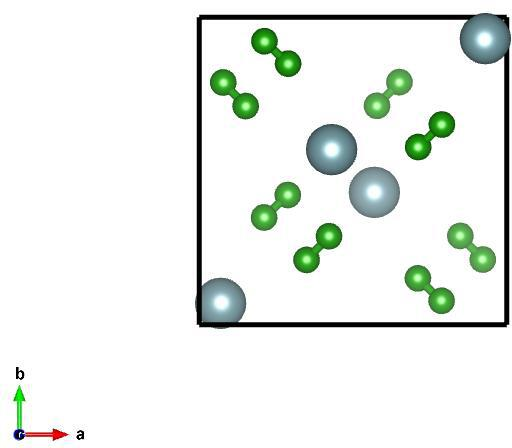
\includegraphics[width=0.9\linewidth,height=2in,keepaspectratio]{/Users/rosecers/work_folders/structures_for_photonics/reference/ref_inp/workspace/dda667e0a39fa5479e6e44fae0f15720/final_images/analog_trim.jpg}\\
\small{Image of \textit{tI}8-YMn\textsubscript{2}, generated by Vesta}
\end{minipage}\hfill
\begin{minipage}{0.65\textwidth}\raggedright
{\setlength{\mathindent}{0cm}
\begin{equation*}
\begin{split}&\boldsymbol{a_1} = -0.5783430911\ \hat{x} + 0.5783430911\ \hat{y} + 0.5753594859\ \hat{z}\\[-8pt]
&\boldsymbol{a_2} = 0.5783430911\ \hat{x} - 0.5783430911\ \hat{y} + 0.5753594859\ \hat{z}\\[-8pt]
&\boldsymbol{a_3} = 0.5783430911\ \hat{x} + 0.5783430911\ \hat{y} - 0.5753594859\ \hat{z}
\end{split}
\end{equation*}}

\textbf{Space Group:}	141\hspace{0.5in}\textbf{Point Group:}	$4/mmm$\\
\textbf{Crystallographic Open Database} \#1524241\\
\textbf{Structure DOI: }\url{10.1088/0953-8984/3/33/023}

\end{minipage}\hfill
\end{figure}
\vspace{-0.25in}


\begin{figure}[H]
\begin{minipage}{0.9\textwidth}\centering
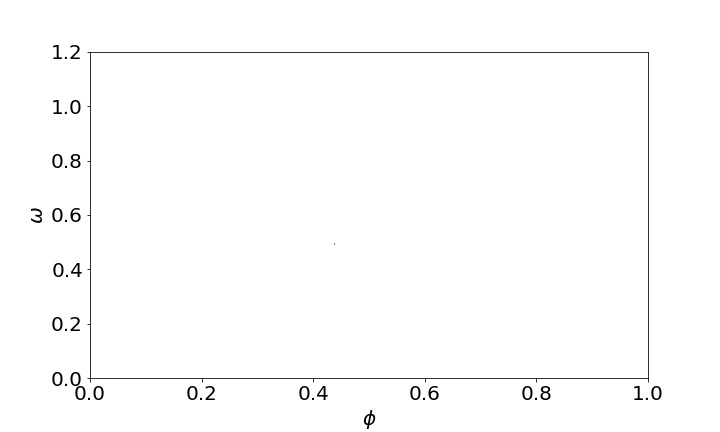
\includegraphics[width=0.9\linewidth,height=2.5in,keepaspectratio]{/Users/rosecers/work_folders/structures_for_photonics/reference/ref_inp/workspace/dda667e0a39fa5479e6e44fae0f15720/final_images/gap_atlas.jpg}
\\
\end{minipage}\hfill\caption{Gap Atlas across filling fraction $\phi$ and frequency $\omega$}
\end{figure}


\begin{figure}[H]
\begin{minipage}{0.5\textwidth}\centering
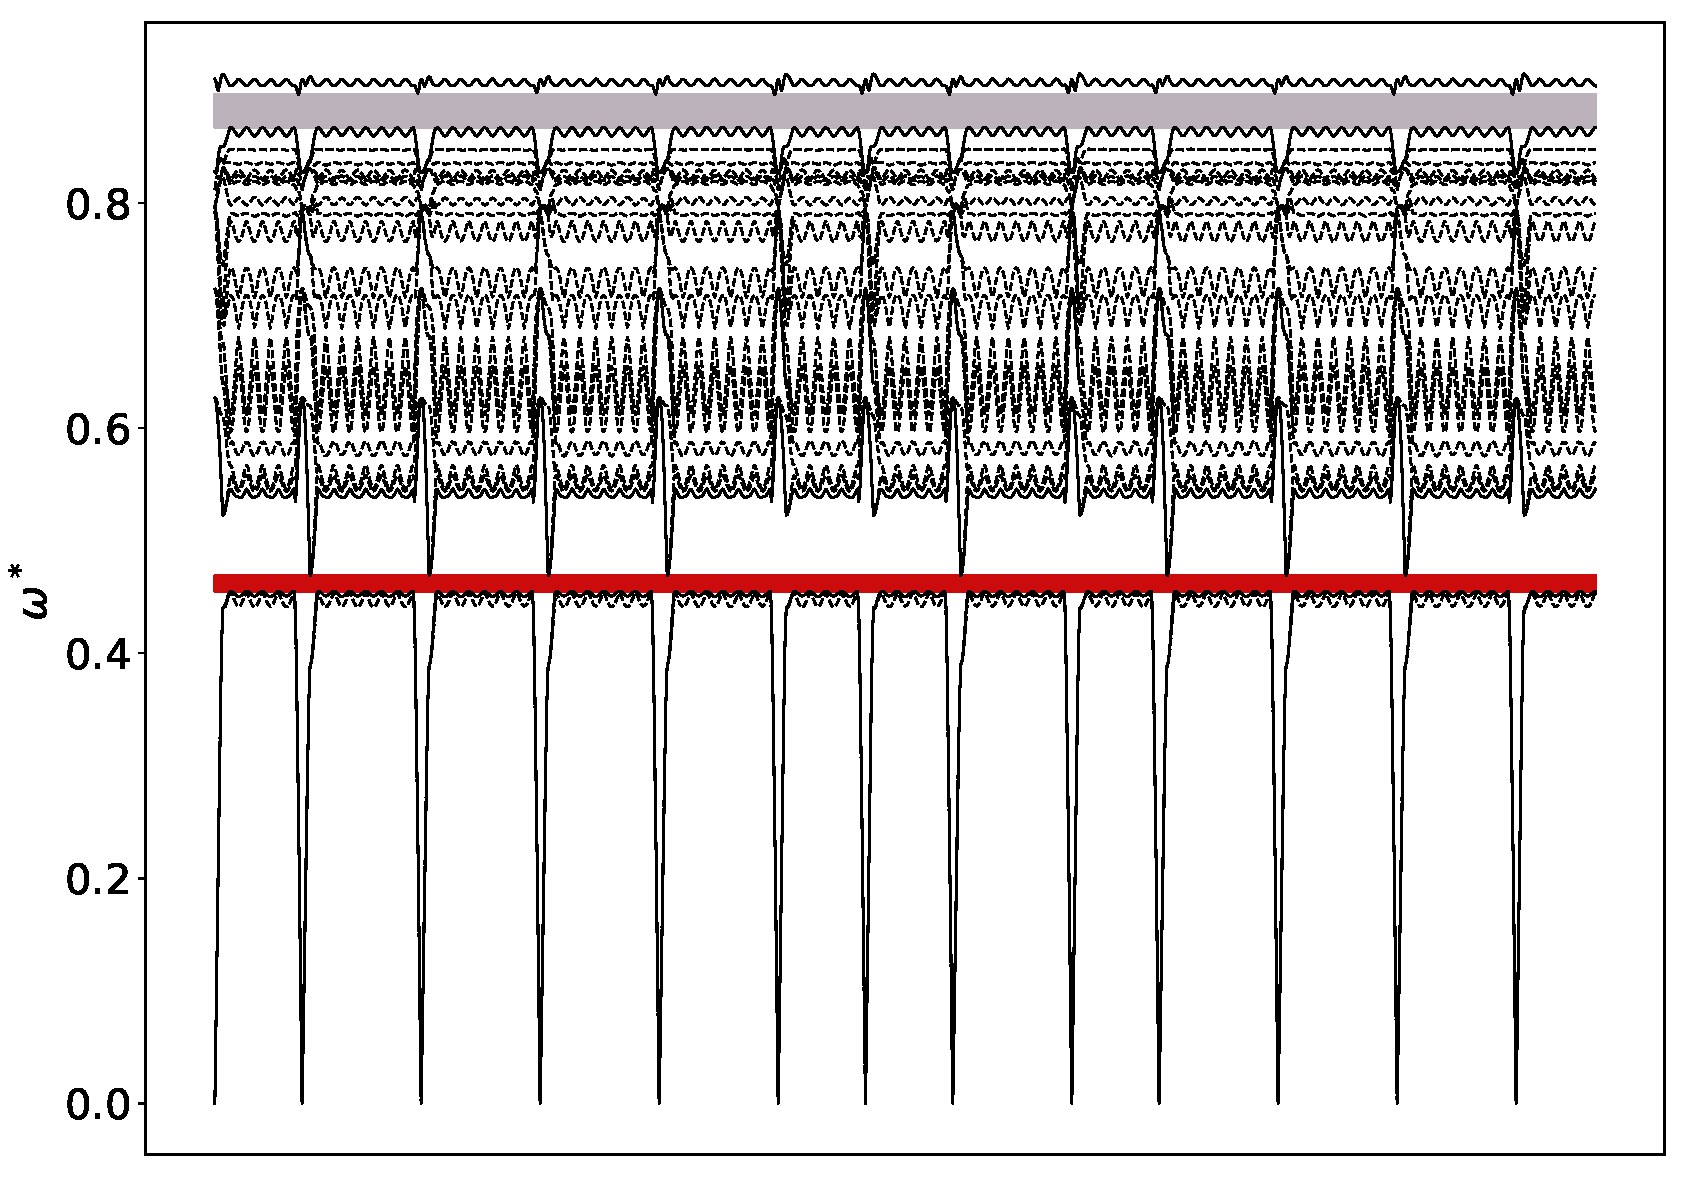
\includegraphics[width=0.9\linewidth,height=2.0in,keepaspectratio]{/Users/rosecers/work_folders/structures_for_photonics/reference/ref_inp/workspace/dda667e0a39fa5479e6e44fae0f15720/./final_images/band_diagram_b=2.pdf}
\\Band Structure across 1st BZ
\end{minipage}\hfill
\begin{minipage}{0.48\textwidth}\centering
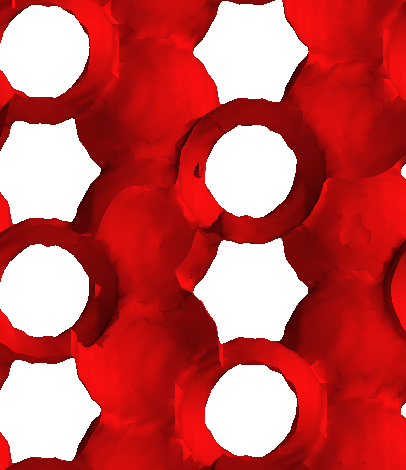
\includegraphics[width=0.9\linewidth,height=2.0in,keepaspectratio]{/Users/rosecers/work_folders/structures_for_photonics/reference/ref_inp/workspace/dda667e0a39fa5479e6e44fae0f15720/final_images/tI8-YMn2@gap_2-3.png}
\\View rotated 45$^{\circ}$ about $l_3$  and elevated 0${\circ}$
\end{minipage}\hfill\caption{Band Structure and Isosurface of \textit{tI}8-YMn\textsubscript{2} (Direct) at radius = 0.29, filling fraction = 0.502, where the largest gap between bands 2 and 3 occurs with gap size 6.01\%.}

\end{figure}
\vspace{-0.25in}


\begin{figure}[H]
\begin{minipage}{0.5\textwidth}\centering
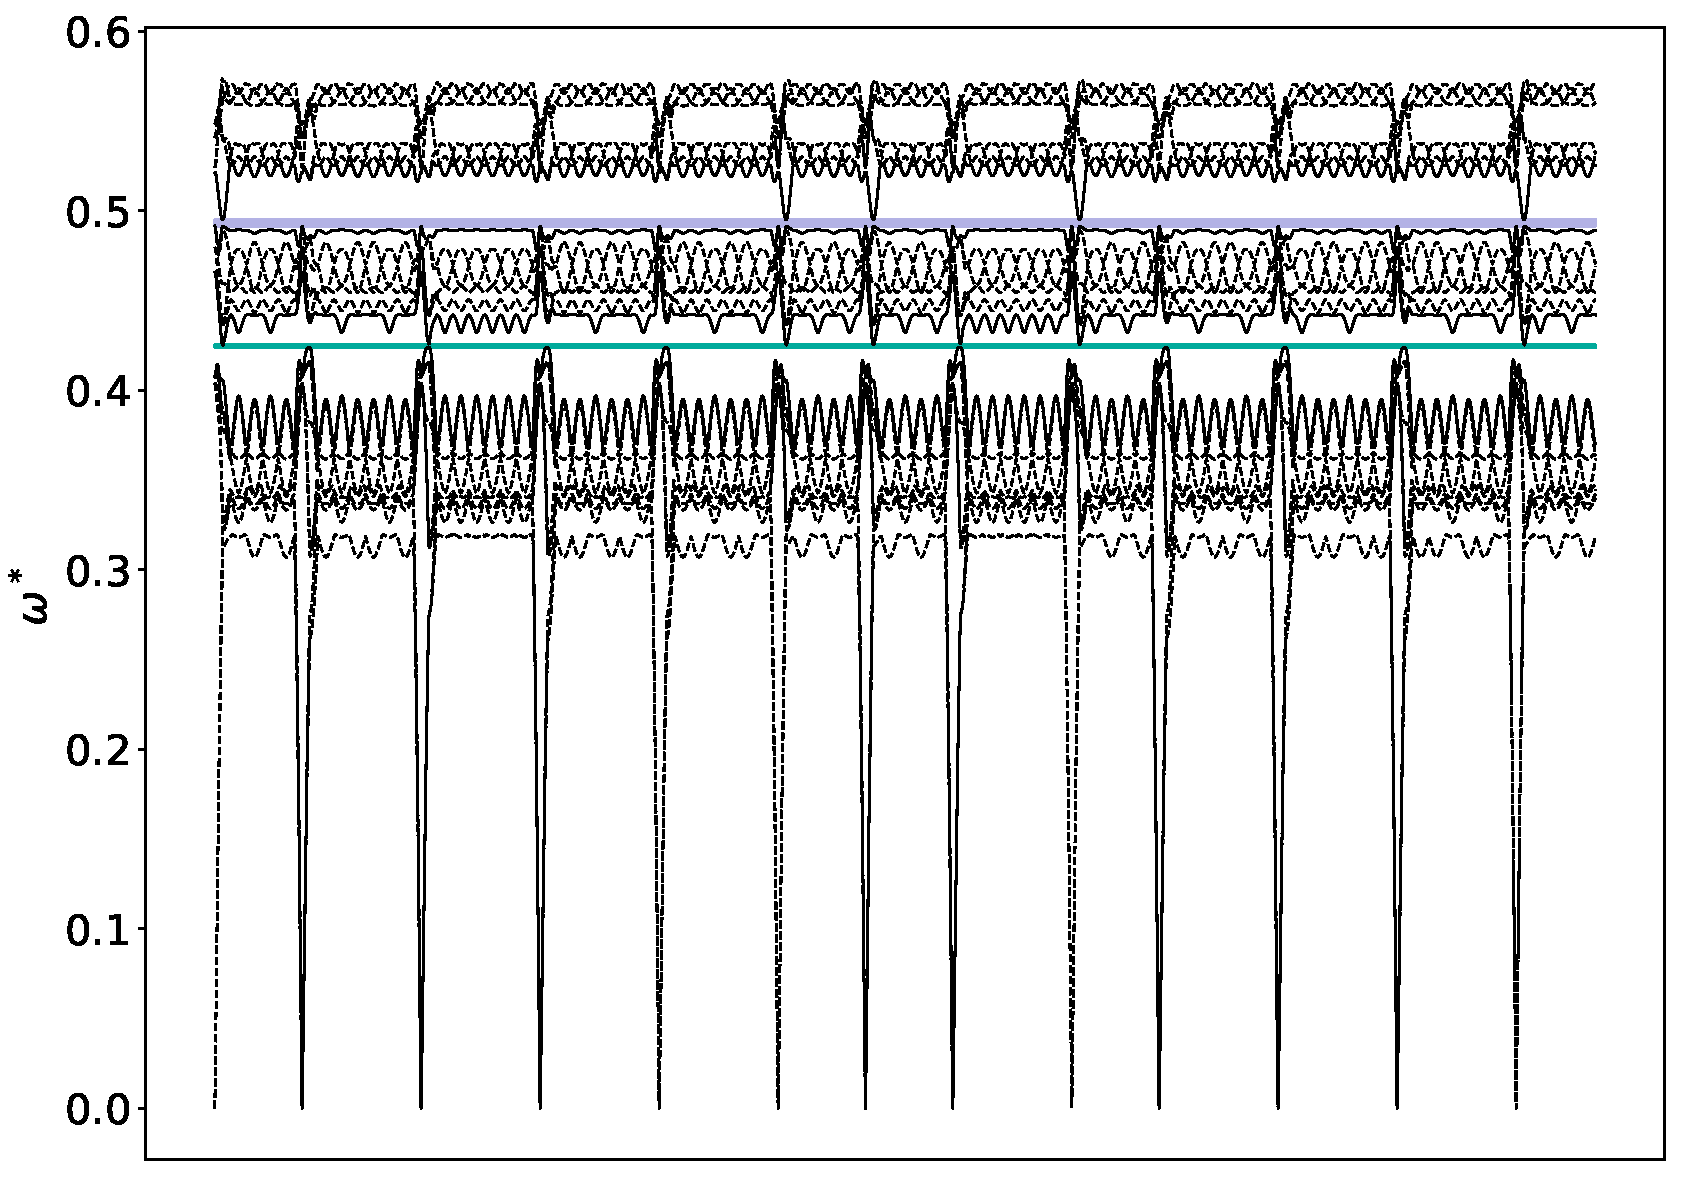
\includegraphics[width=0.9\linewidth,height=2.0in,keepaspectratio]{/Users/rosecers/work_folders/structures_for_photonics/reference/ref_inp/workspace/dda667e0a39fa5479e6e44fae0f15720/./final_images/band_diagram_b=14.pdf}
\\Band Structure across 1st BZ
\end{minipage}\hfill
\begin{minipage}{0.48\textwidth}\centering
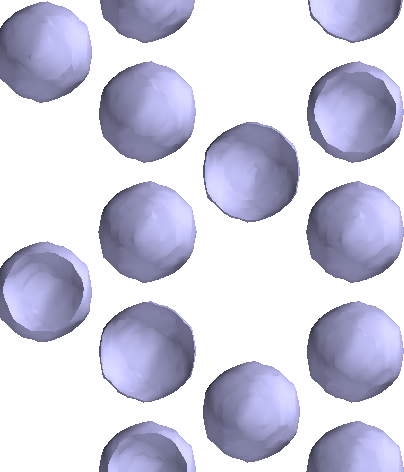
\includegraphics[width=0.9\linewidth,height=2.0in,keepaspectratio]{/Users/rosecers/work_folders/structures_for_photonics/reference/ref_inp/workspace/dda667e0a39fa5479e6e44fae0f15720/final_images/tI8-YMn2@gap_14-15.png}
\\View along $a_1$ 
\end{minipage}\hfill\caption{Band Structure and Isosurface of \textit{tI}8-YMn\textsubscript{2} (Direct) at radius = 0.2, filling fraction = 0.174, where the largest gap between bands 14 and 15 occurs with gap size 4.82\%.}

\end{figure}
\vspace{-0.25in}

